\documentclass[journal]{IEEEtran}
\usepackage[a5paper, margin=10mm]{geometry}
%\usepackage{lmodern} % Ensure lmodern is loaded for pdflatex
\usepackage{tfrupee} % Include tfrupee package


\setlength{\headheight}{1cm} % Set the height of the header box
\setlength{\headsep}{0mm}     % Set the distance between the header box and the top of the text


%\usepackage[a5paper, top=10mm, bottom=10mm, left=10mm, right=10mm]{geometry}

%
\setlength{\intextsep}{10pt} % Space between text and floats

\makeindex


\usepackage{cite}
\usepackage{amsmath,amssymb,amsfonts,amsthm}
\usepackage{algorithmic}
\usepackage{graphicx}
\usepackage{textcomp}
\usepackage{xcolor}
\usepackage{txfonts}
\usepackage{listings}
\usepackage{enumitem}
\usepackage{mathtools}
\usepackage{gensymb}
\usepackage{comment}
\usepackage[breaklinks=true]{hyperref}
\usepackage{tkz-euclide} 
\usepackage{listings}
\usepackage{multicol}
\usepackage{xparse}
\usepackage{gvv}
%\def\inputGnumericTable{}                                 
\usepackage[latin1]{inputenc}                                
\usepackage{color}                                            
\usepackage{array}                                            
\usepackage{longtable}                                       
\usepackage{calc}                                             
\usepackage{multirow}                                         
\usepackage{hhline}                                           
\usepackage{ifthen}                                               
\usepackage{lscape}
\usepackage{tabularx}
\usepackage{array}
\usepackage{float}
\usepackage{ar}
\usepackage[version=4]{mhchem}


\newtheorem{theorem}{Theorem}[section]
\newtheorem{problem}{Problem}
\newtheorem{proposition}{Proposition}[section]
\newtheorem{lemma}{Lemma}[section]
\newtheorem{corollary}[theorem]{Corollary}
\newtheorem{example}{Example}[section]
\newtheorem{definition}[problem]{Definition}
\newcommand{\BEQA}{\begin{eqnarray}}
\newcommand{\EEQA}{\end{eqnarray}}

\theoremstyle{remark}


\begin{document}
\bibliographystyle{IEEEtran}
\onecolumn

\title{1.9.16}
\author{INDHIRESH S- EE25BTECH11027}
\maketitle


\renewcommand{\thefigure}{\theenumi}
\renewcommand{\thetable}{\theenumi}

\textbf{Question} Find the distance between the points $(a, b)$ and $(-a, -b)$.\\
\textbf{Solution}:\\
Let us solve the given equation theoretically and then verify the solution computationally. \\
Let the given two points be P and Q, where,
\begin{align}
    \Vec{P}=\myvec{a\\b} \; and\; \Vec{Q}=\myvec{-a\\-b}
\end{align}
Let D be a vector defined as:
\begin{align}
 \Vec{D}=\vec{P}-\Vec{Q}   
\end{align}
Now,
\begin{align}
    \vec{D}=\myvec{a\\b}-\myvec{-a\\-b}
\end{align}
\begin{align}
    \Vec{D}=\myvec{2a\\2b}
\end{align}
The distance between the point P and Q $=$ Norm of the vector D\\
Norm of the vector D is defined as:
\begin{align}
    ||D||\triangleq\sqrt{D^TD}
\end{align}
\begin{align}
    D^TD=\myvec{2a&2b}\myvec{2a\\2b}
\end{align}
\begin{align}
    D^TD=4a^2+4b^2
\end{align}
Now substituite in Eq.5:
\begin{align}
    ||D||=\sqrt{4a^2+4b^2}
\end{align}
\begin{align}
    ||D||=2\sqrt{a^2+b^2}
\end{align}
Therefore the distance between the two points is:    $2\sqrt{a^2+b^2}$\\\\
For verification let us assume $a=4\;and\; b=4$\\
From the figure it is clearly verified that the theoretical solution matches with the computational solution.\\
\begin{figure}[h]
    \centering
    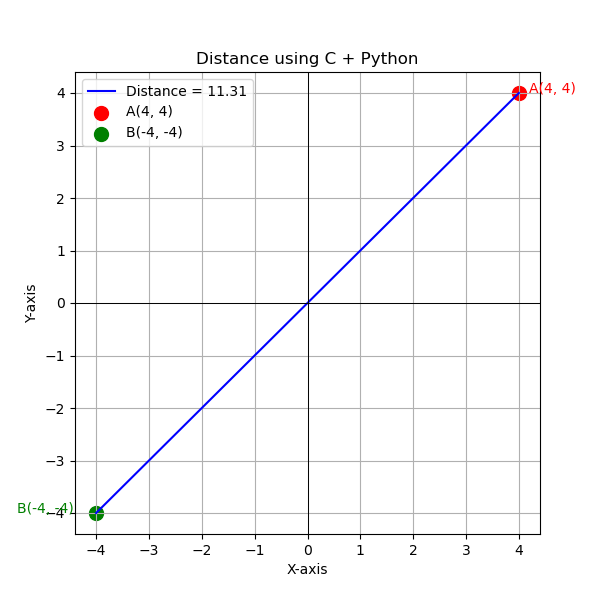
\includegraphics[height=0.5\textheight, keepaspectratio]{figs/figure1.png}
    \label{figure_1}
\end{figure}

\end{document}
\end{document}
